% !TEX root = slides.tex

\section{Introduction}

\begin{frame}{Introduction}
    \only<1>{
        \begin{figure}
            \centering
            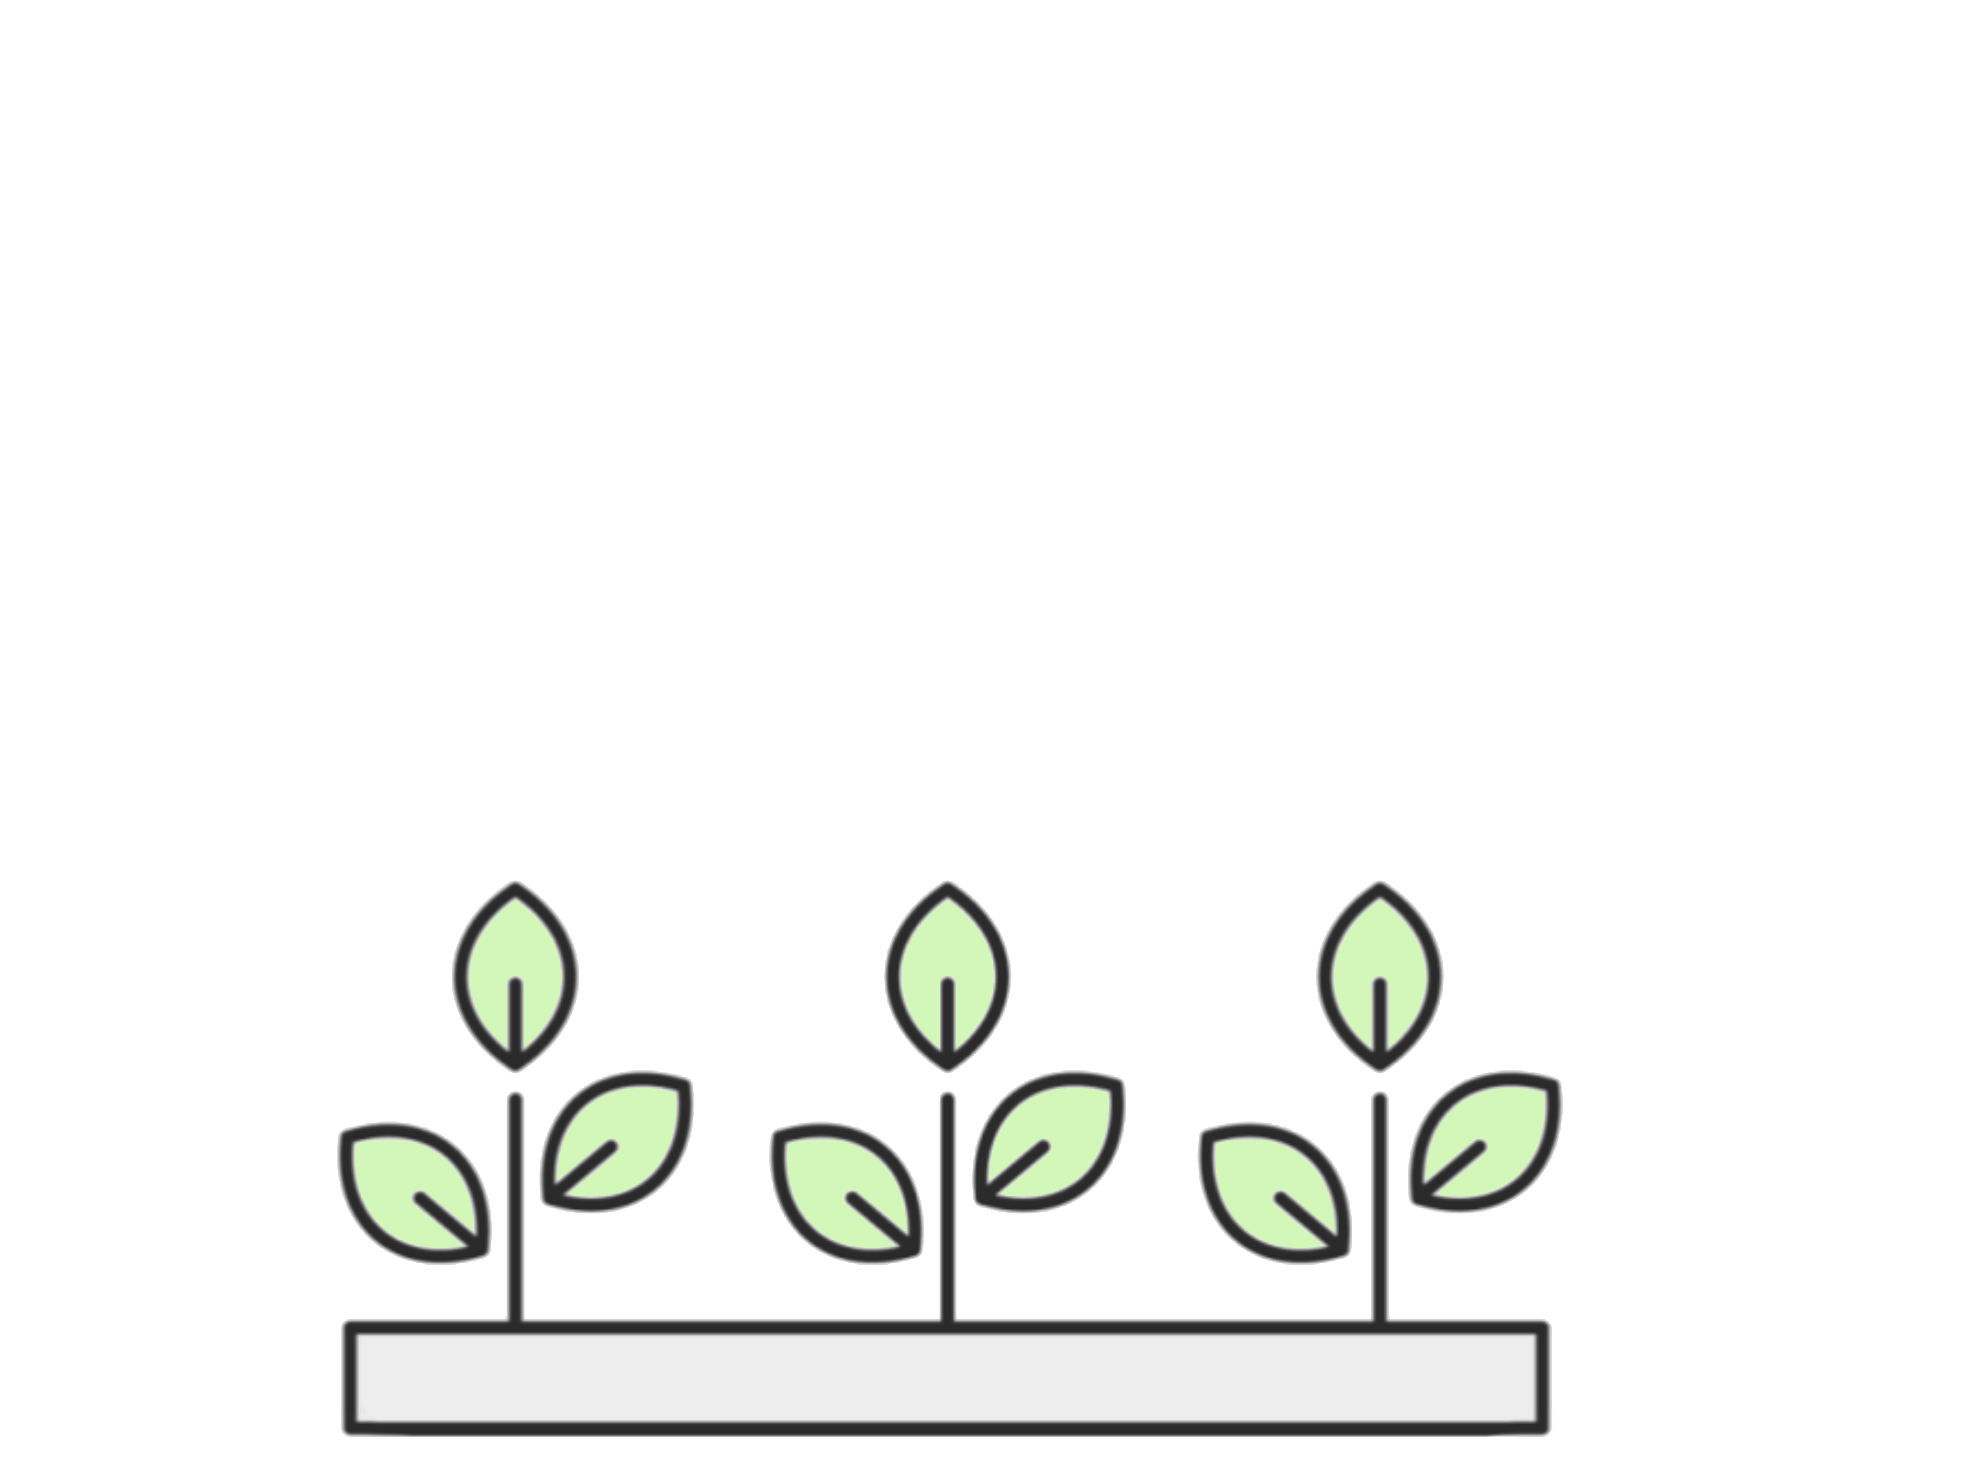
\includegraphics[scale=0.2]{figures/1_plants.png}
        \end{figure}
    }
    \only<2>{
        \begin{figure}
            \centering
            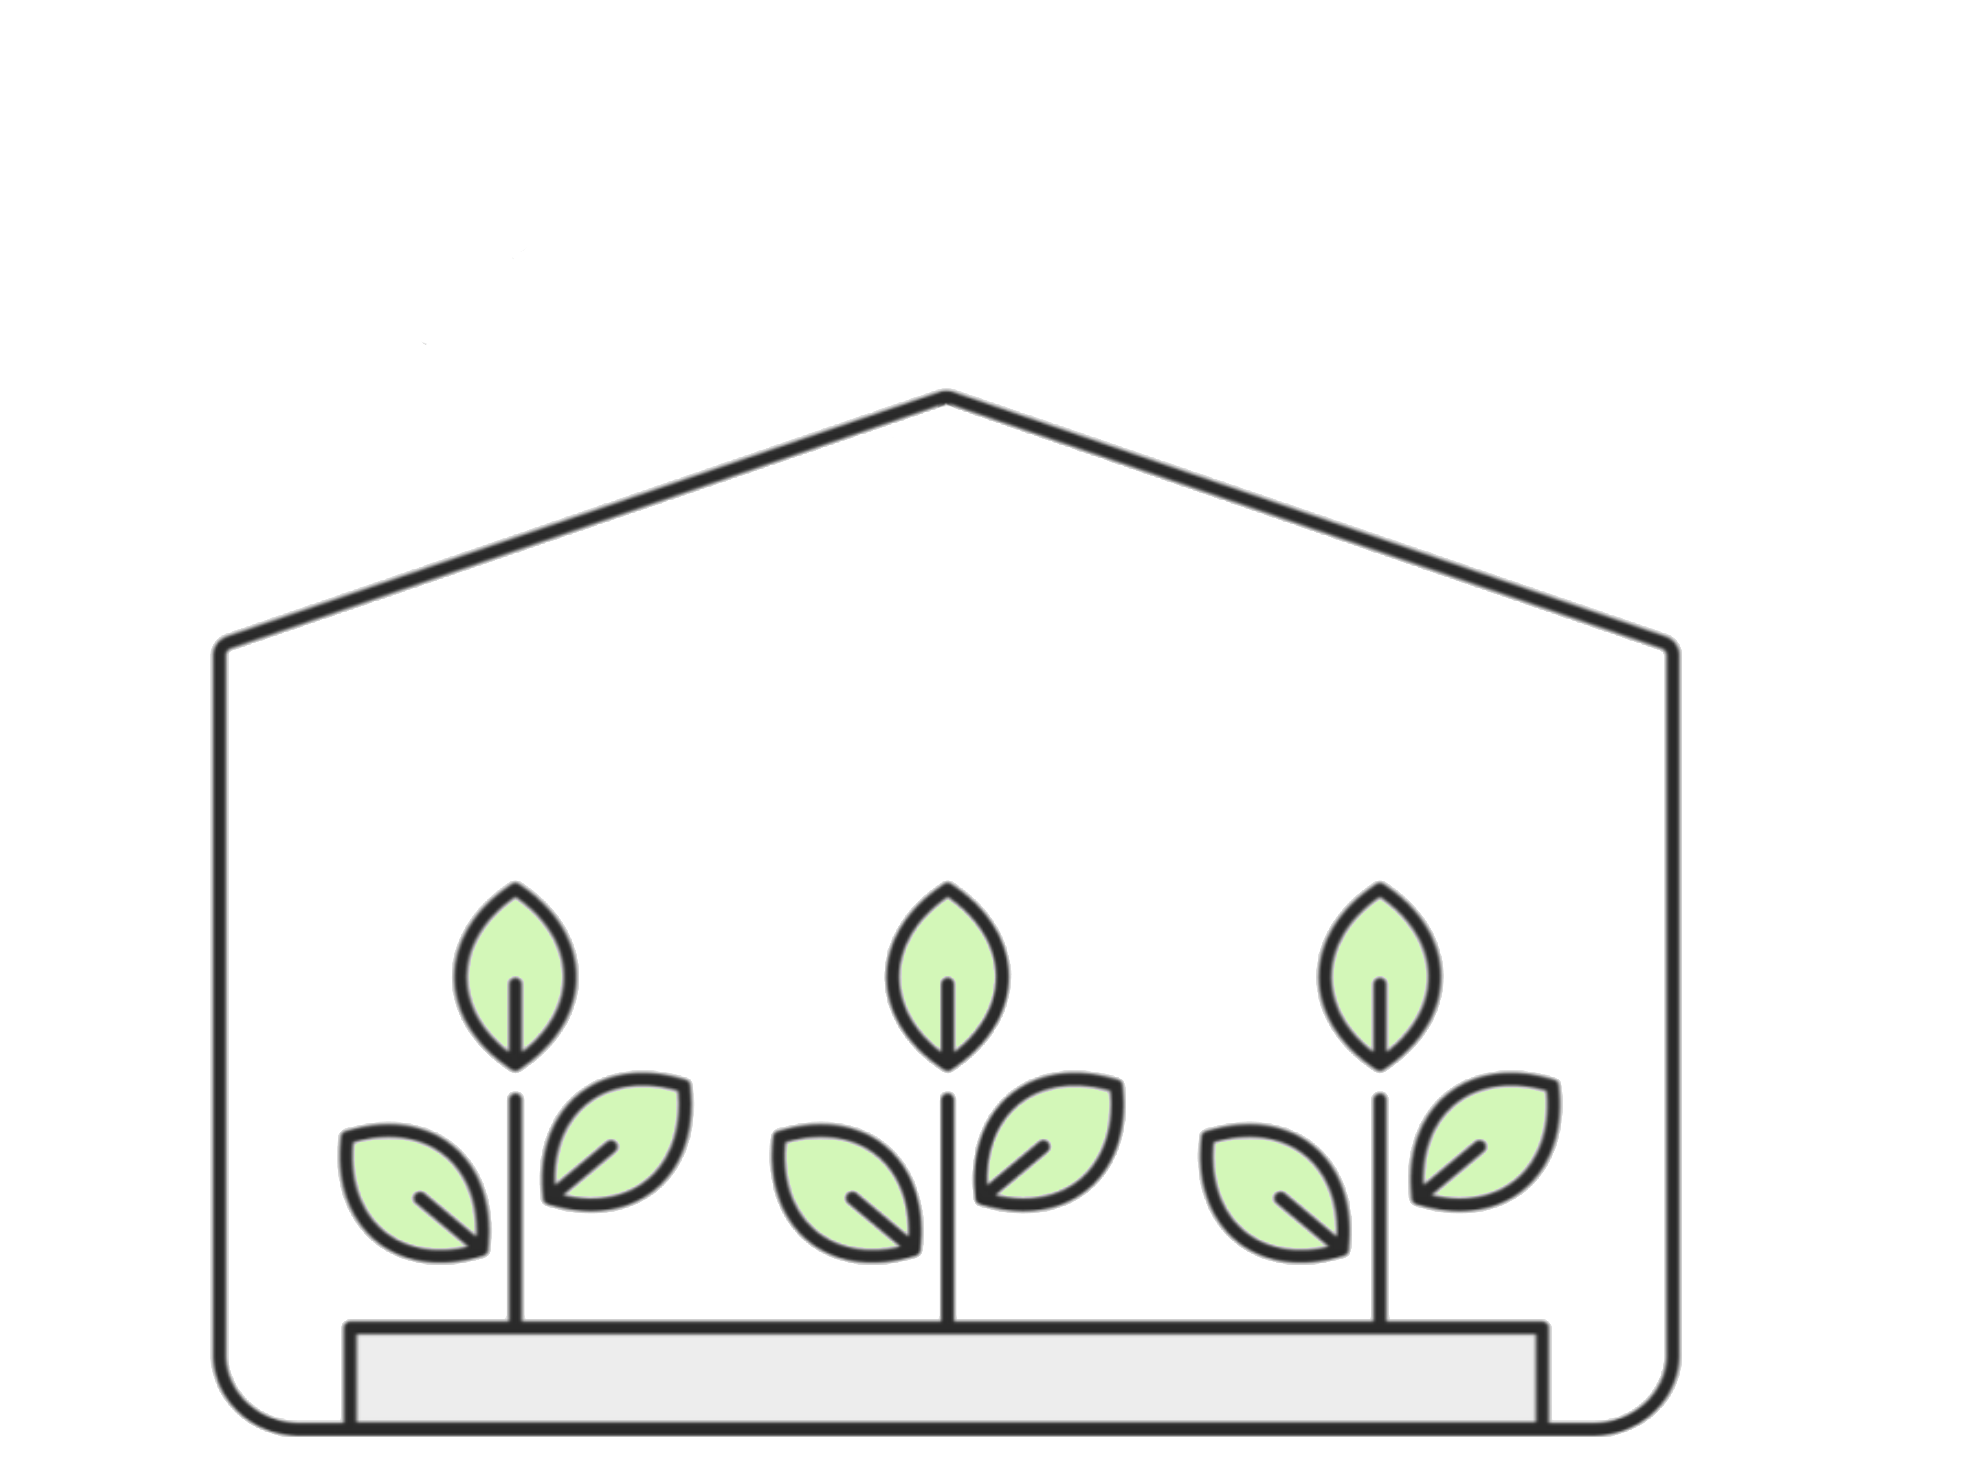
\includegraphics[scale=0.2]{figures/2_greenhouse.png}
        \end{figure}
    }
    \only<3>{
        \begin{figure}
            \centering
            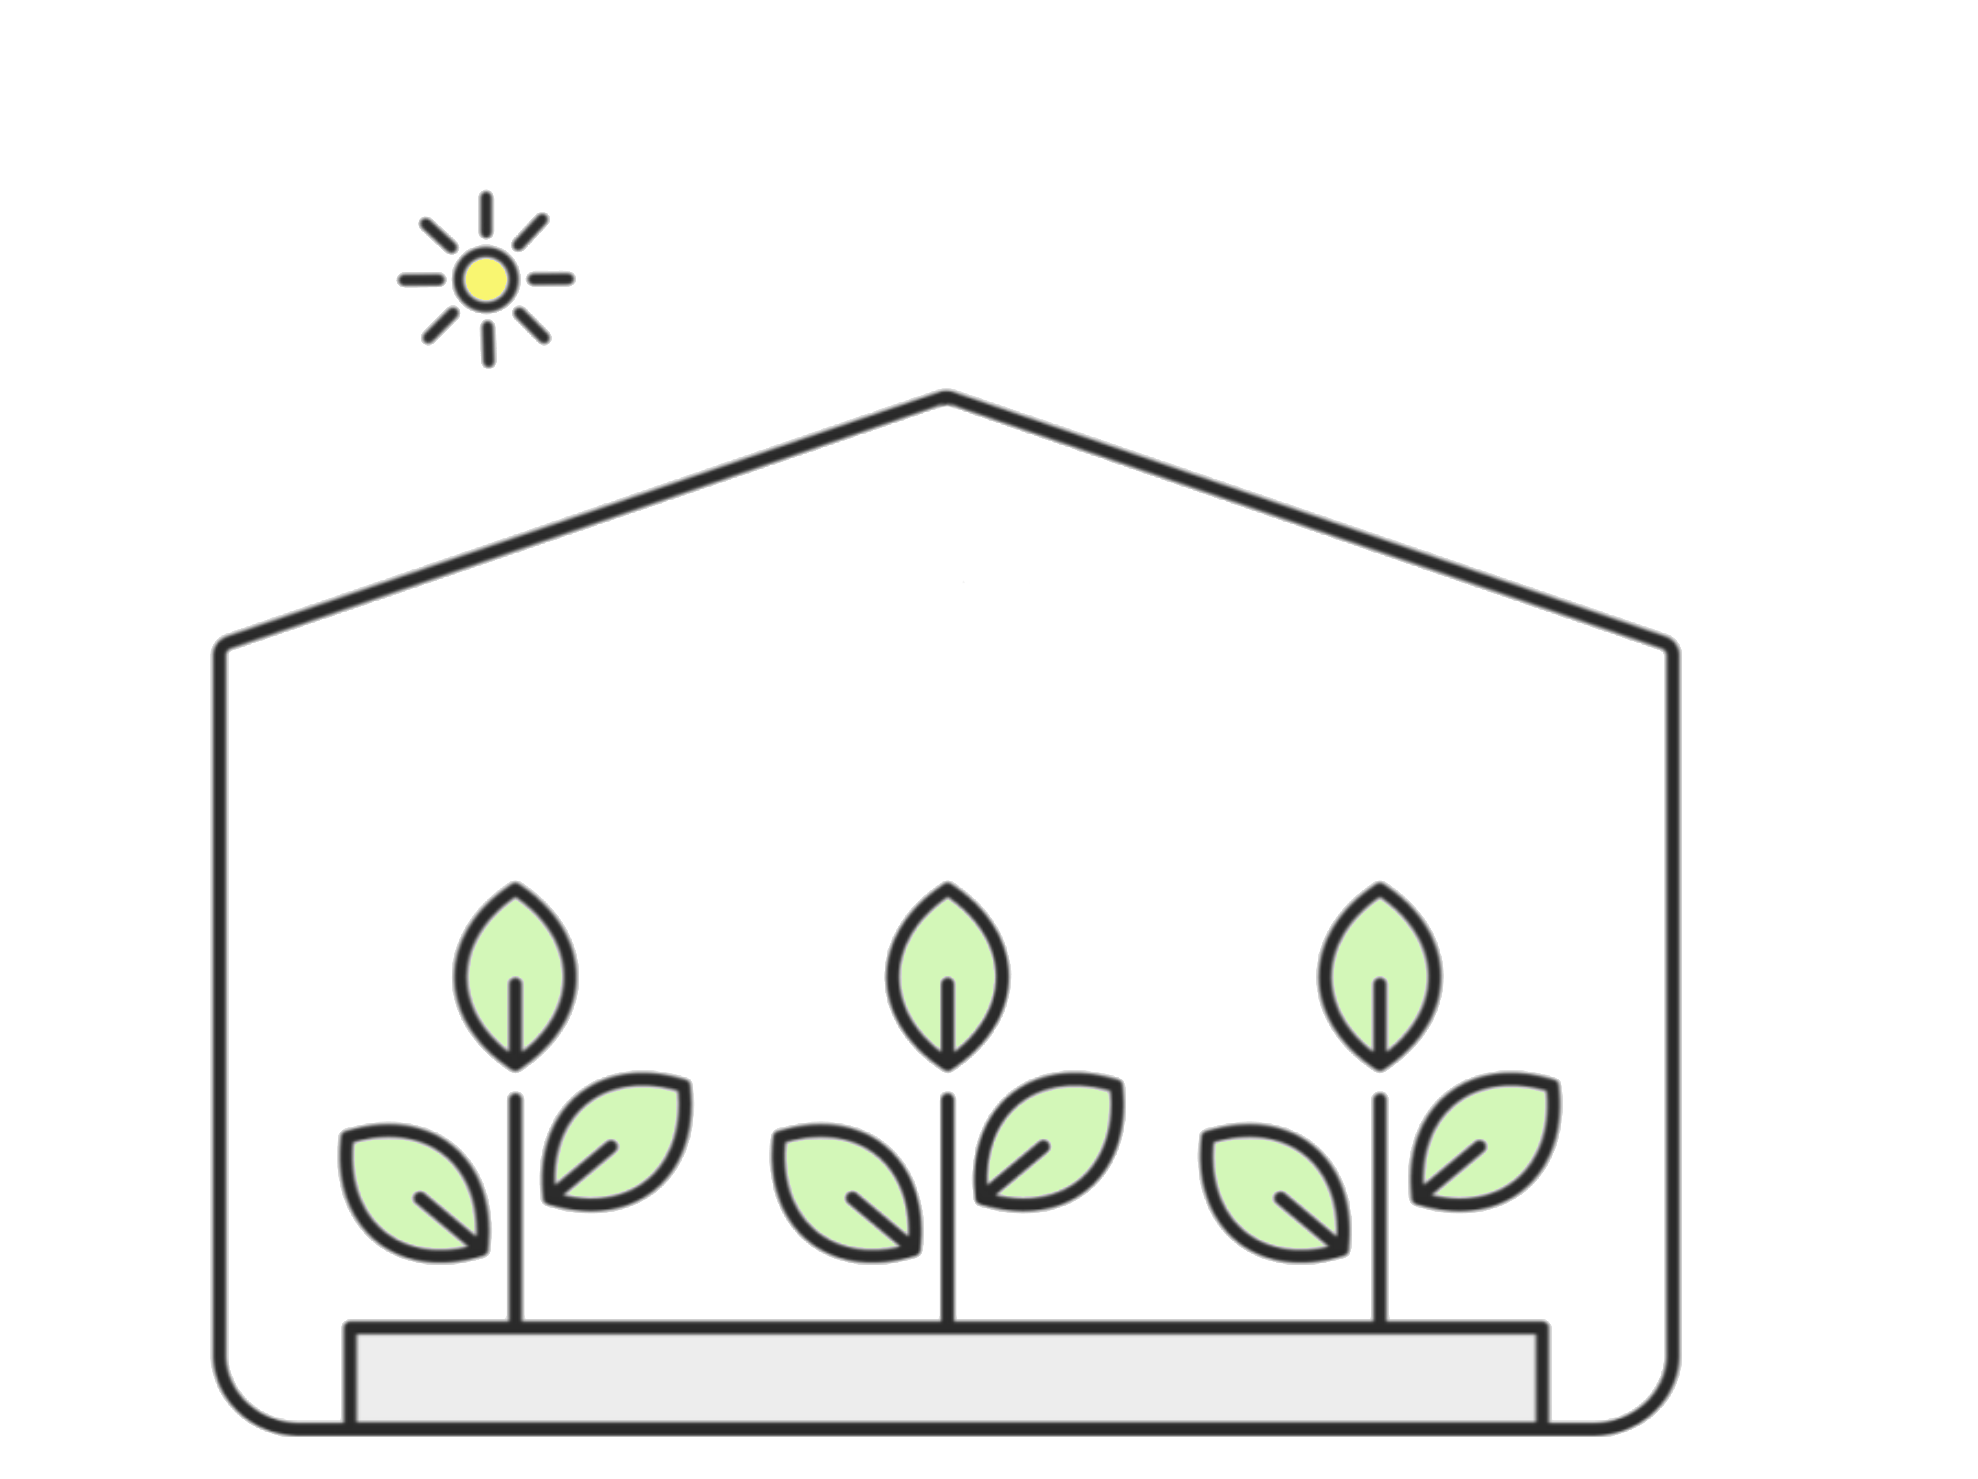
\includegraphics[scale=0.2]{figures/3_sun.png}
        \end{figure}
    }
    \only<4>{
        \begin{figure}
            \centering
            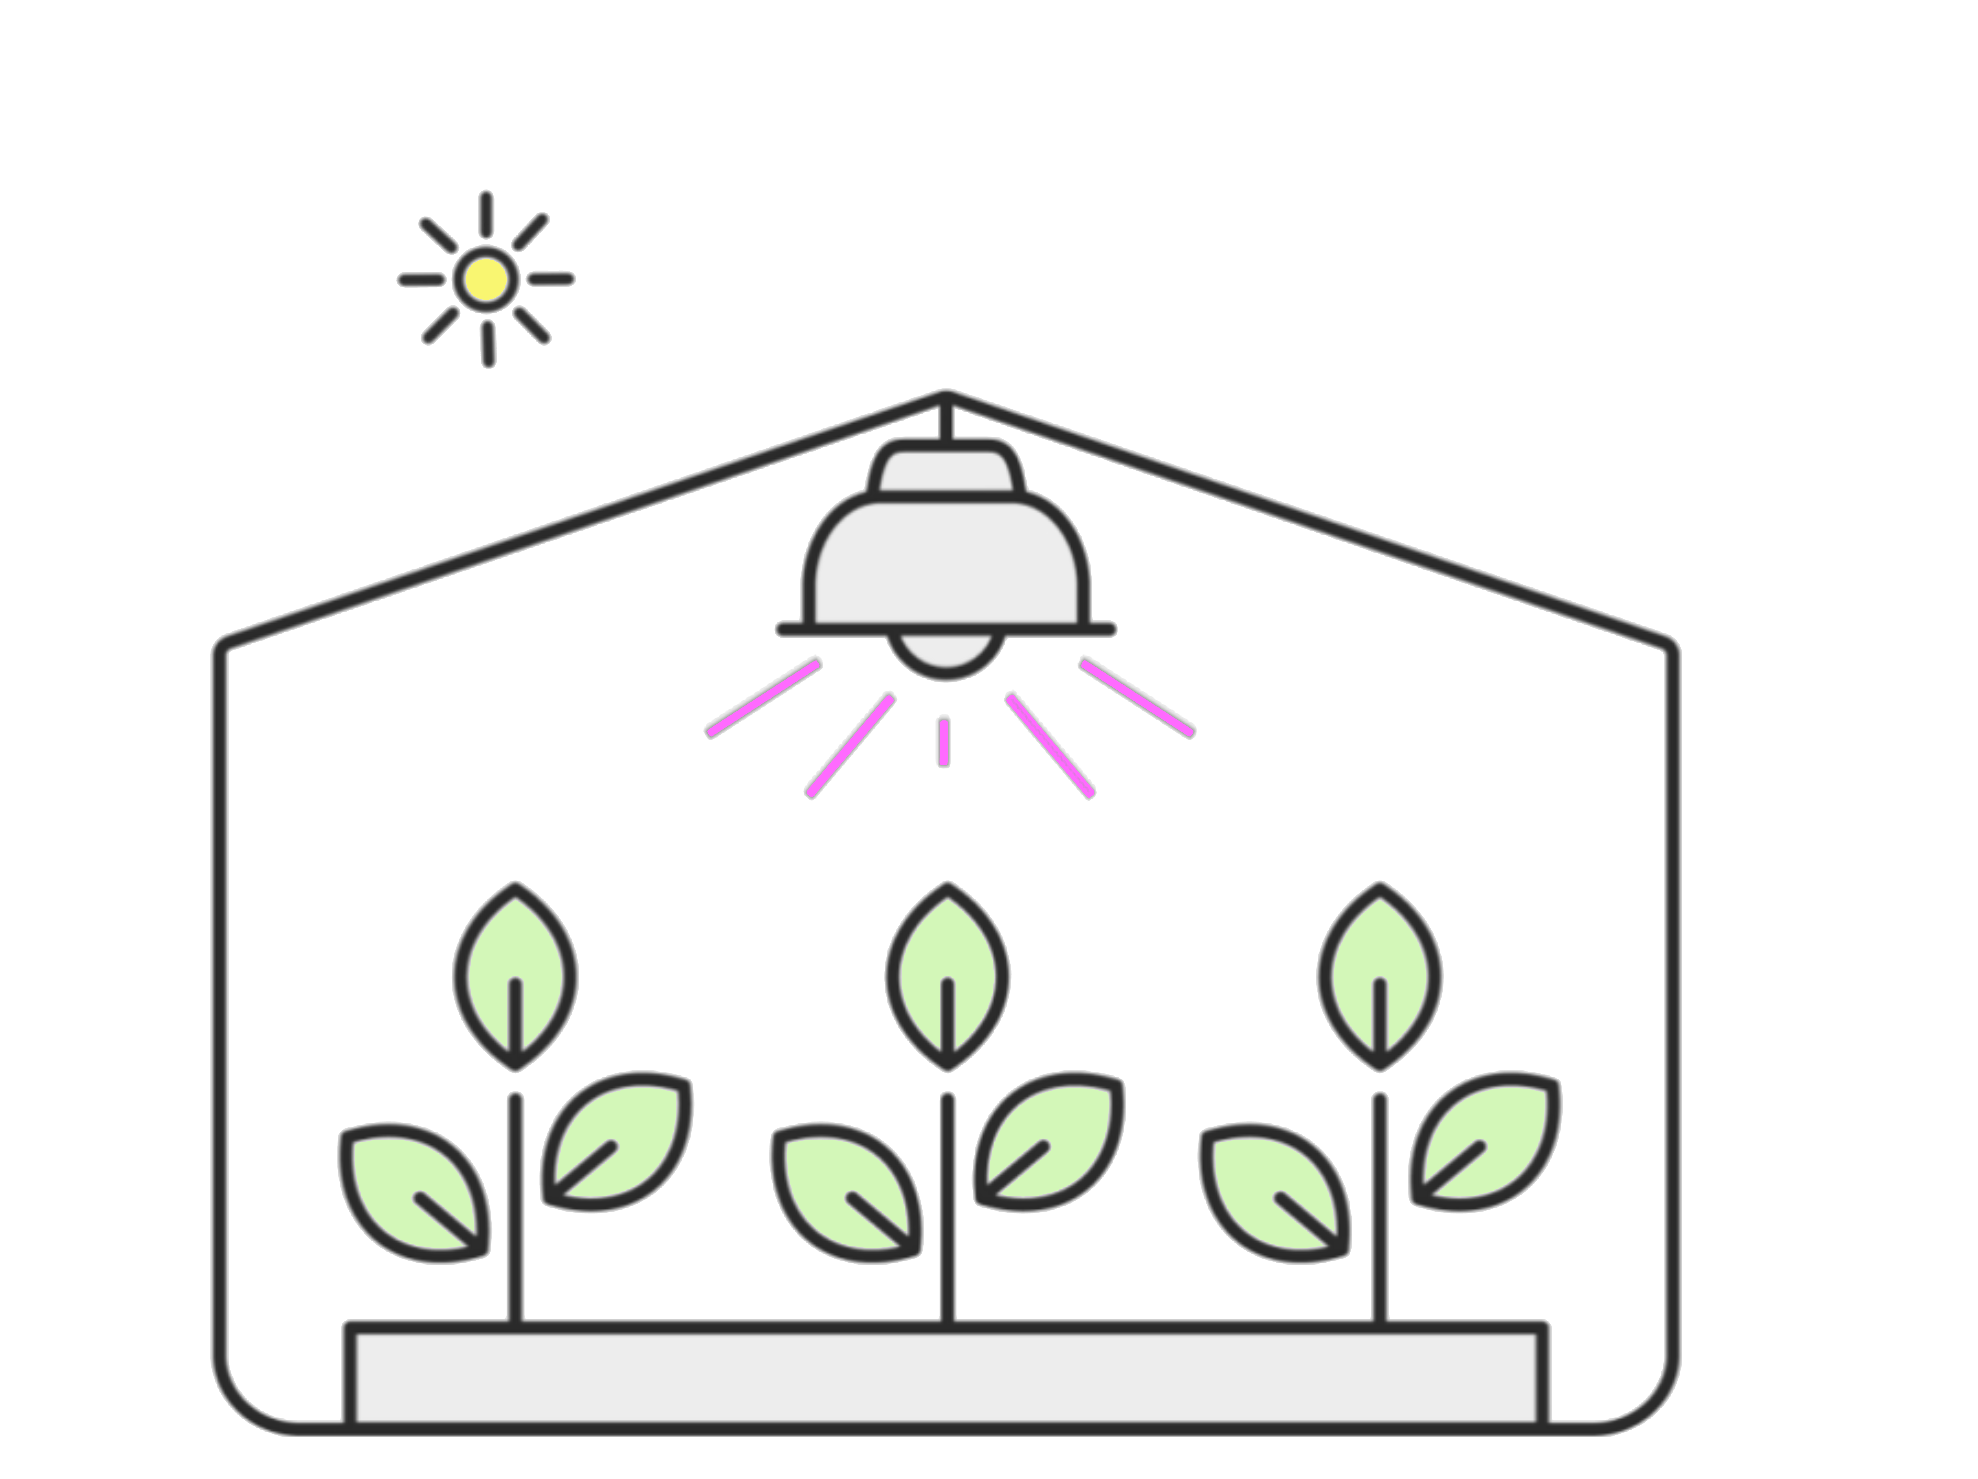
\includegraphics[scale=0.2]{figures/4_lights.png}
        \end{figure}
    }
    \only<5>{
        \begin{figure}
            \centering
            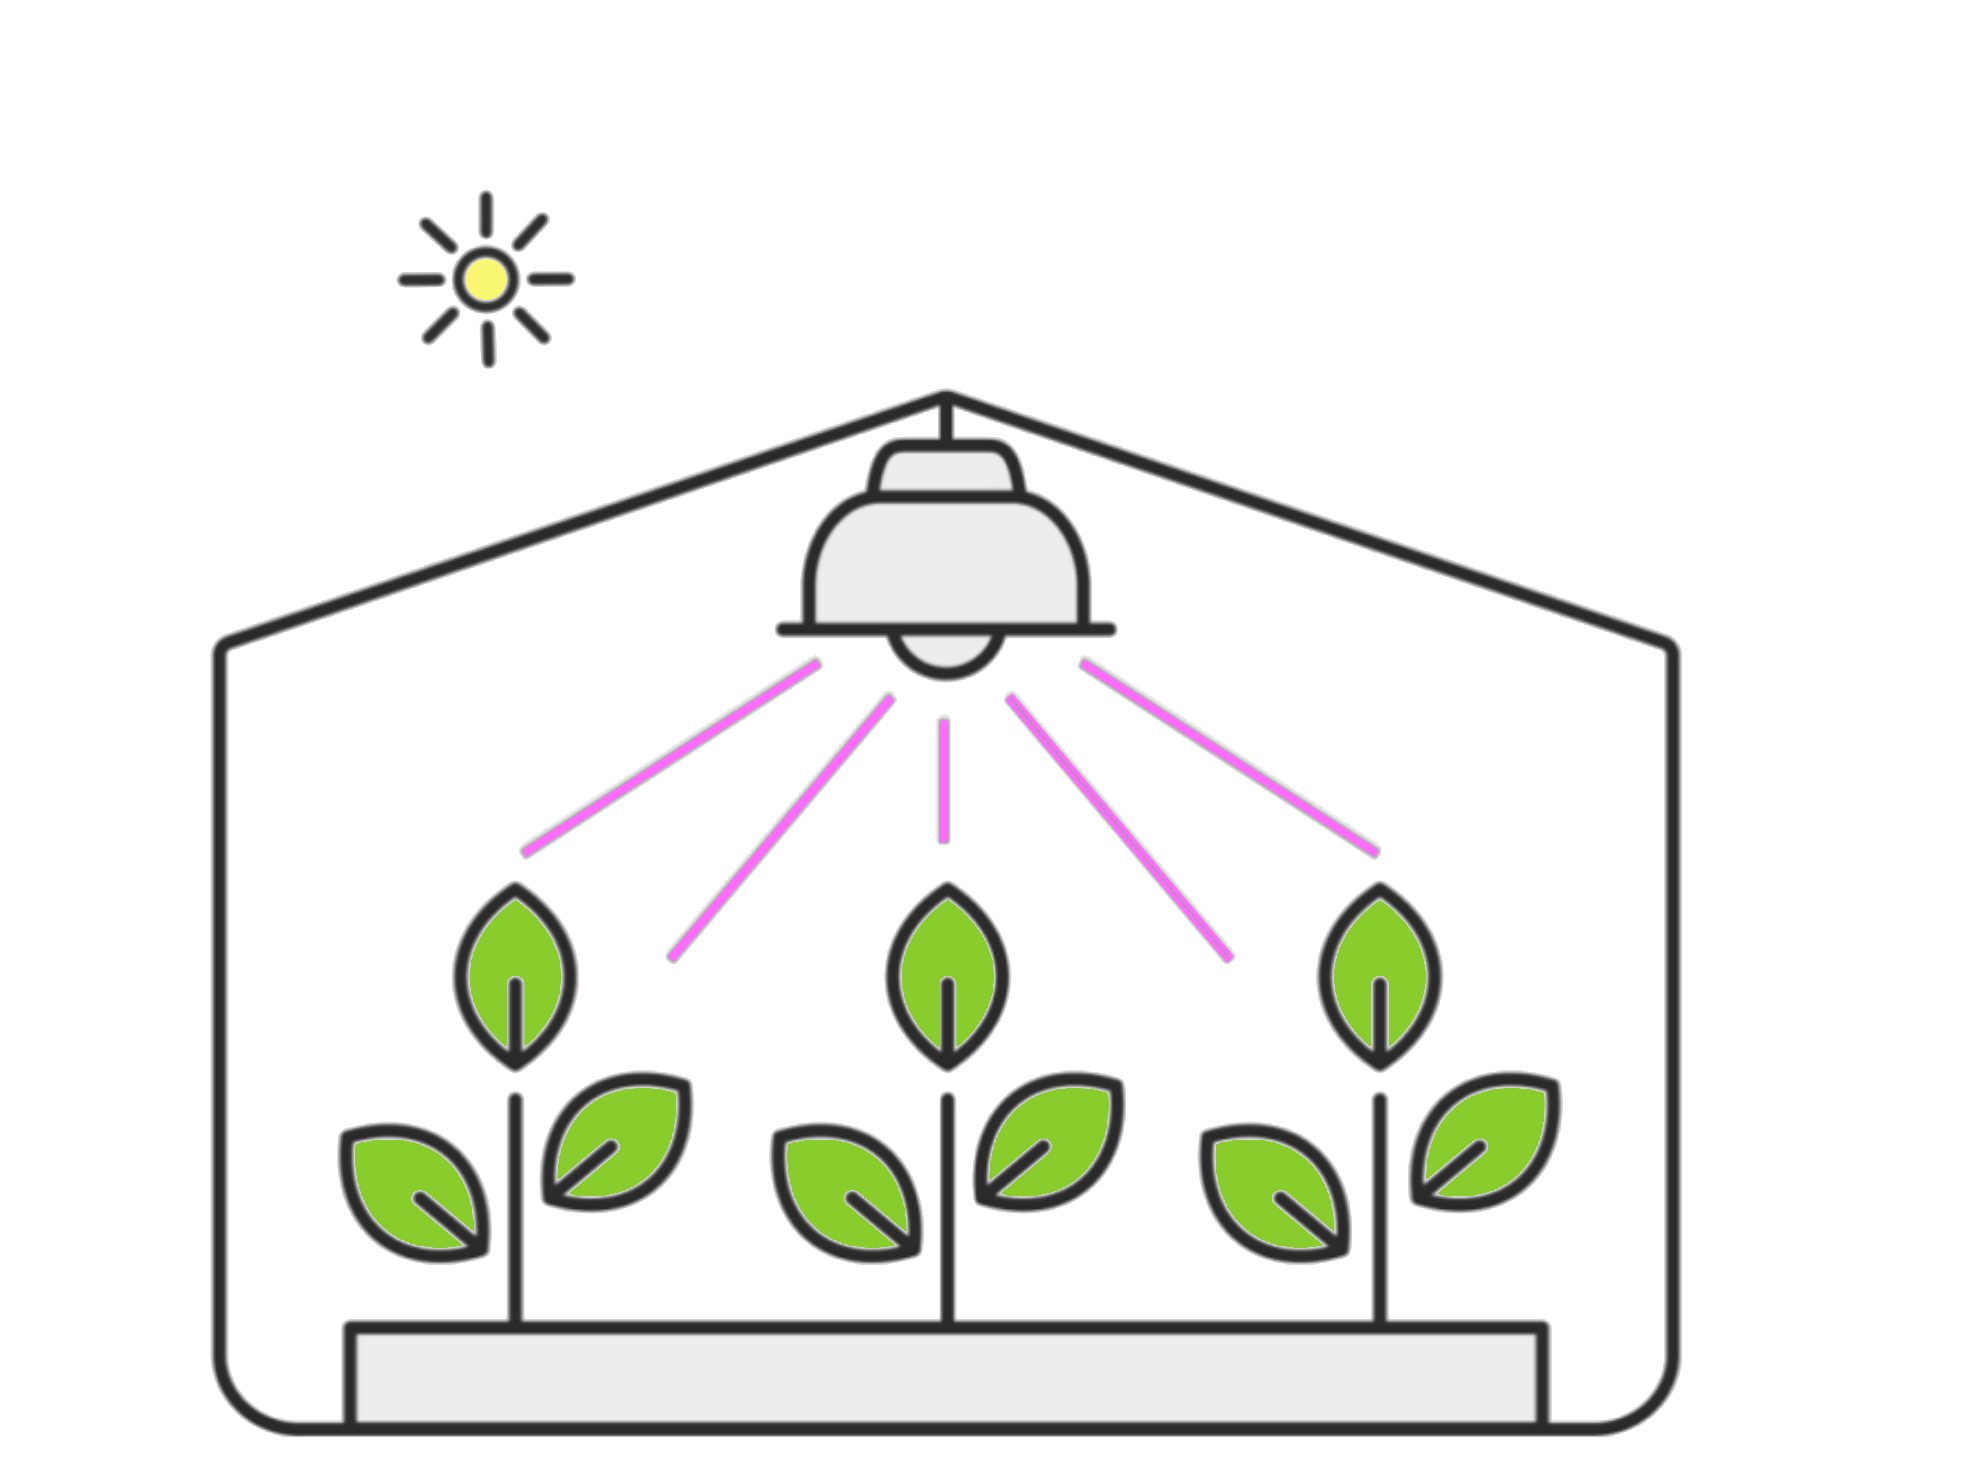
\includegraphics[scale=0.2]{figures/5_photosynthesis.png}
        \end{figure}
    }
    \only<6>{
        \begin{figure}
            \centering
            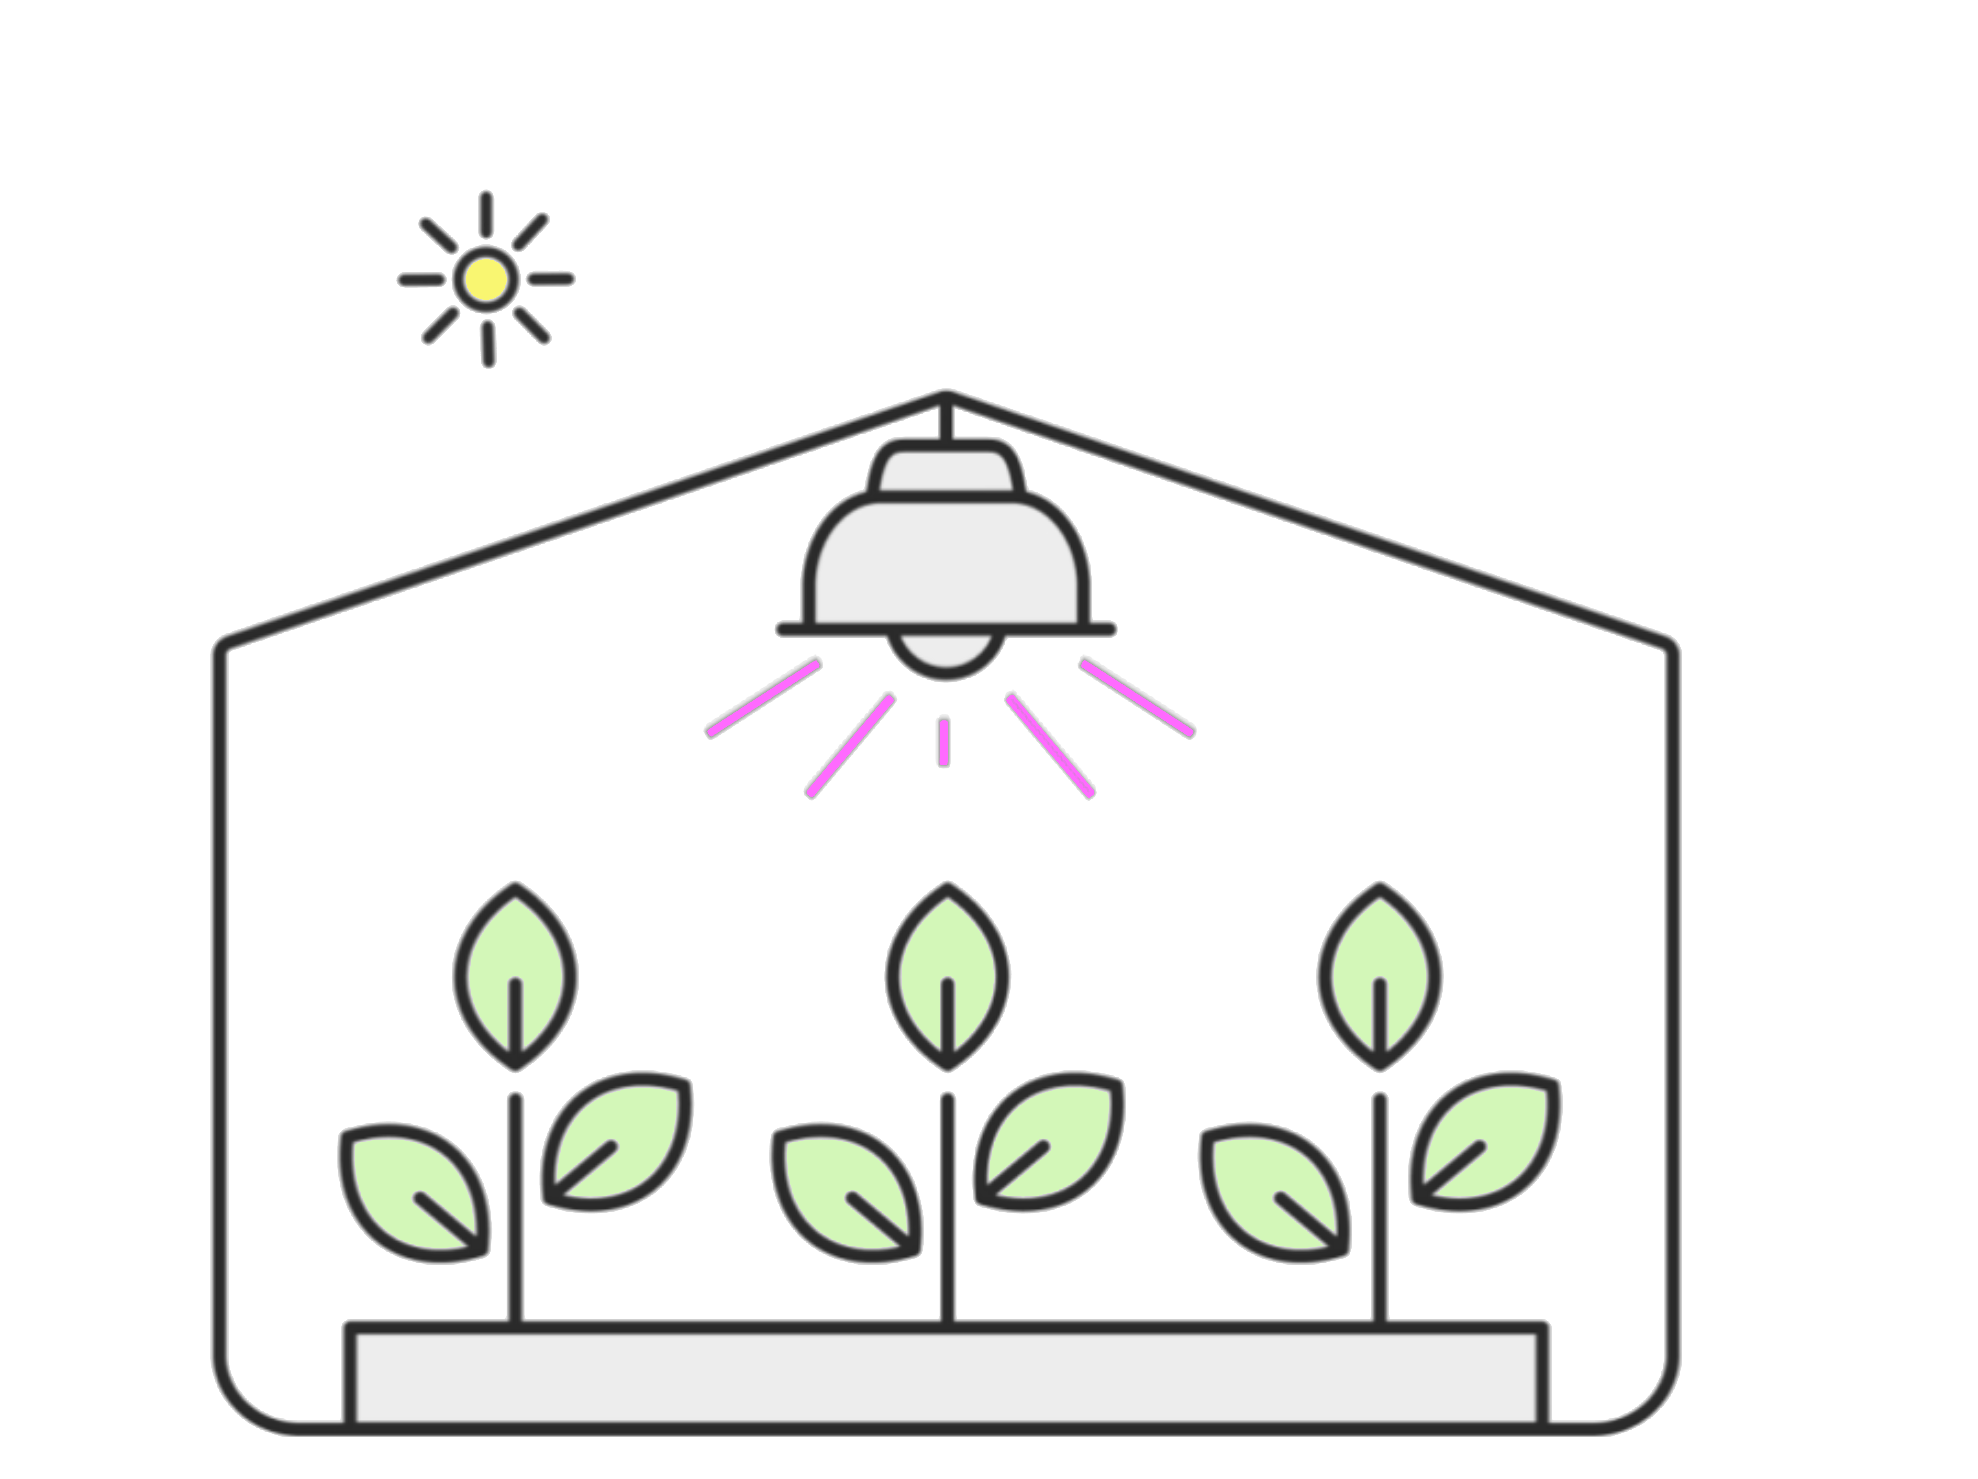
\includegraphics[scale=0.2]{figures/4_lights.png}
        \end{figure}
    }
    \only<7>{
        \begin{columns}
            \begin{column}{0.5\textwidth}
                \begin{figure}
                    \centering
                    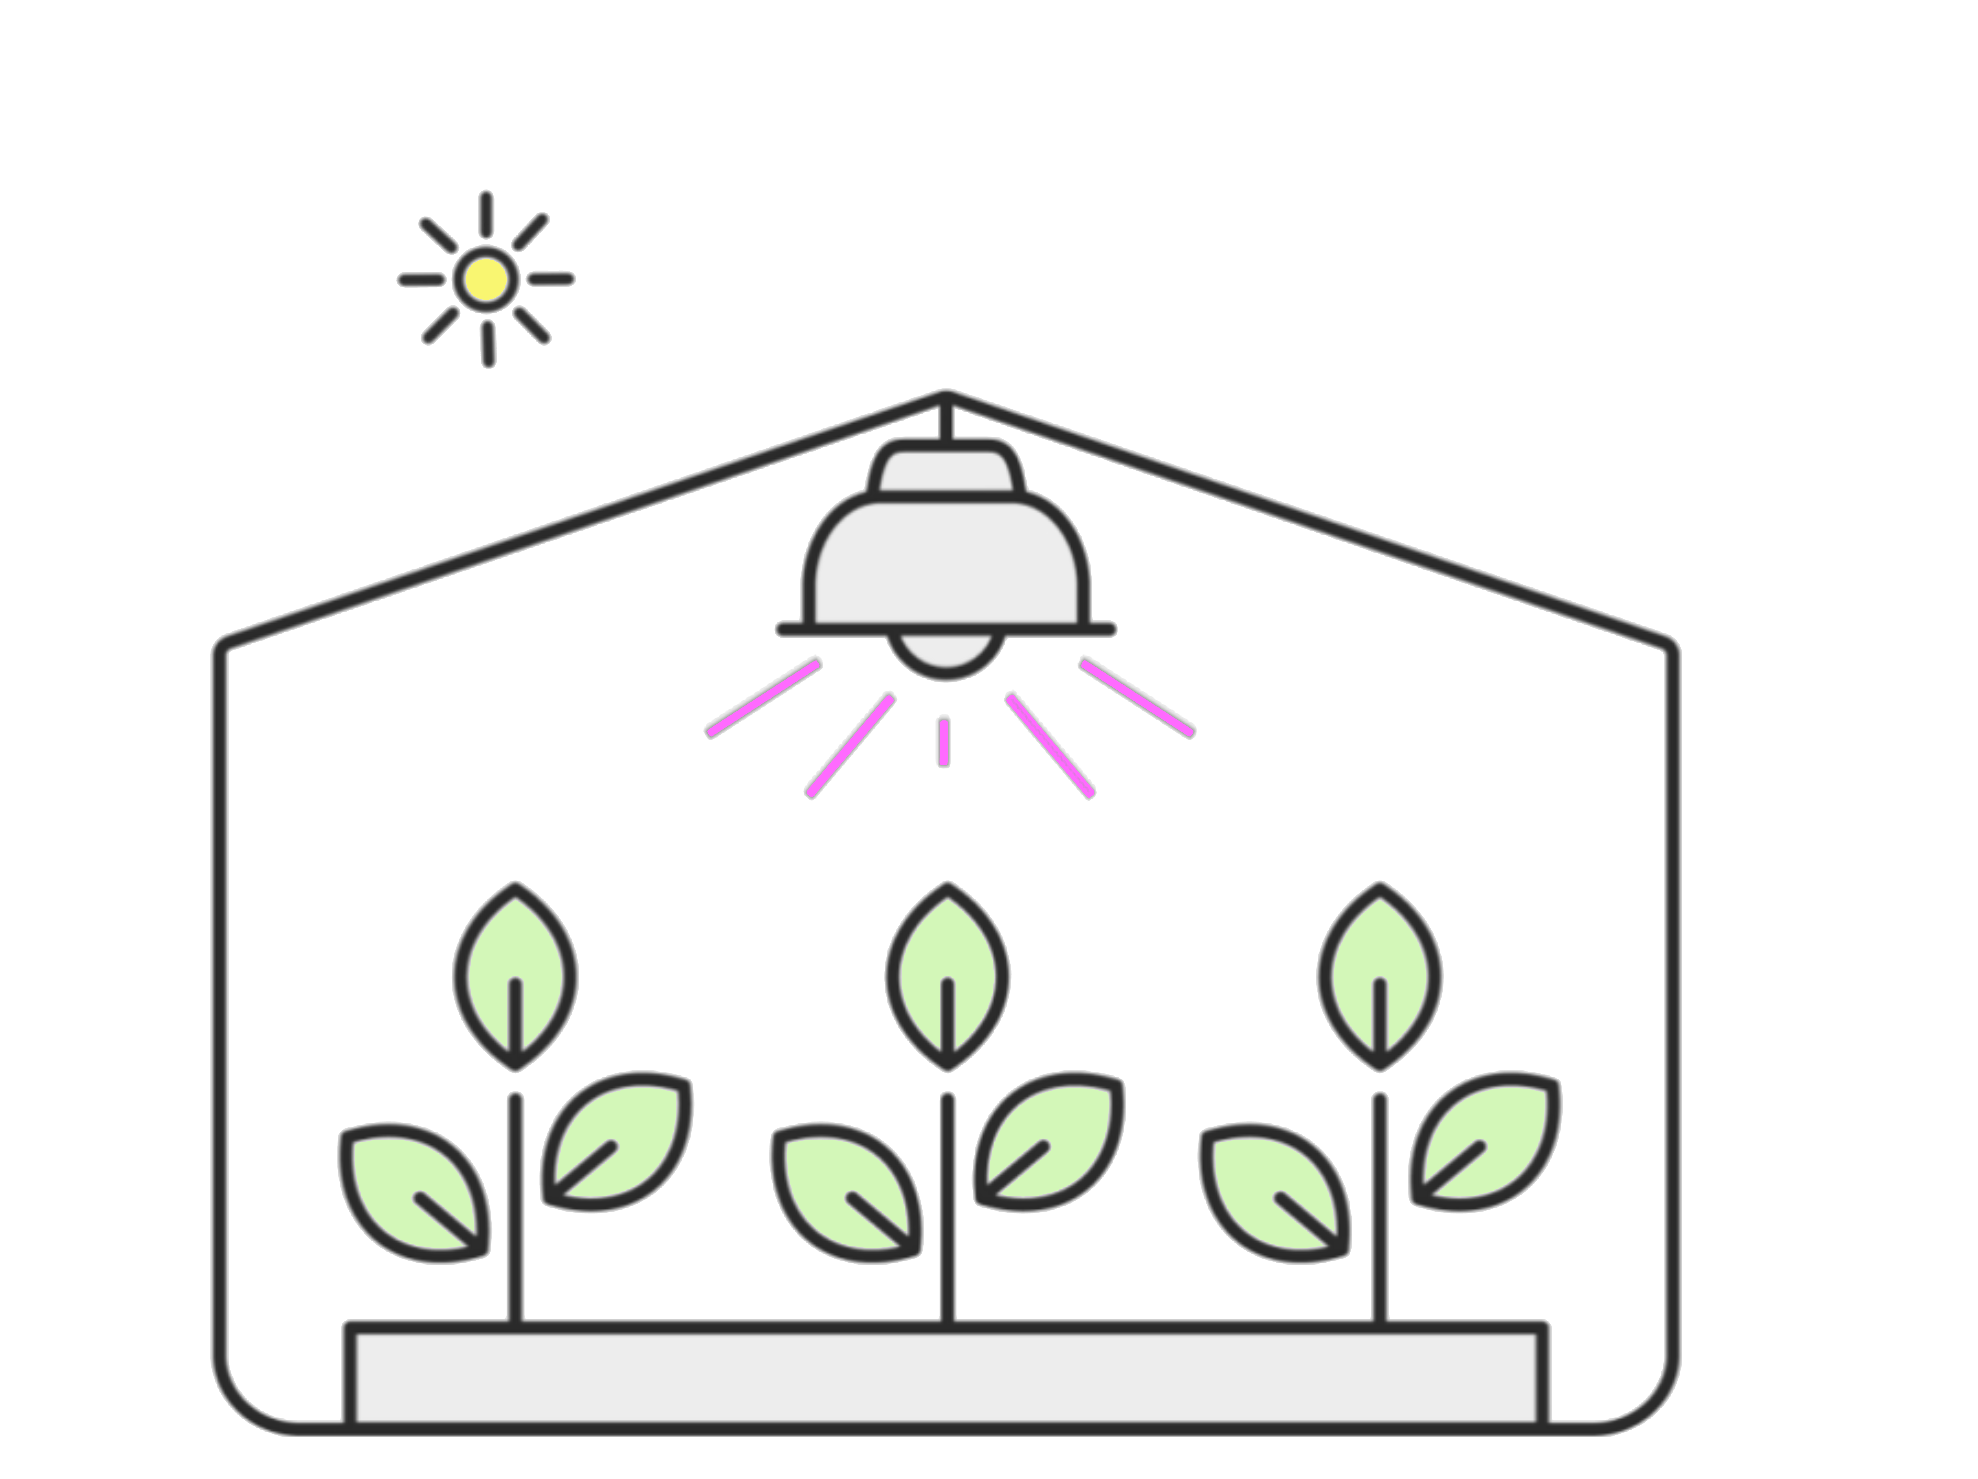
\includegraphics[scale=0.175]{figures/4_lights.png}
                \end{figure}
            \end{column}
            \begin{column}{0.5\textwidth}
                \begin{figure}
                    \centering
                    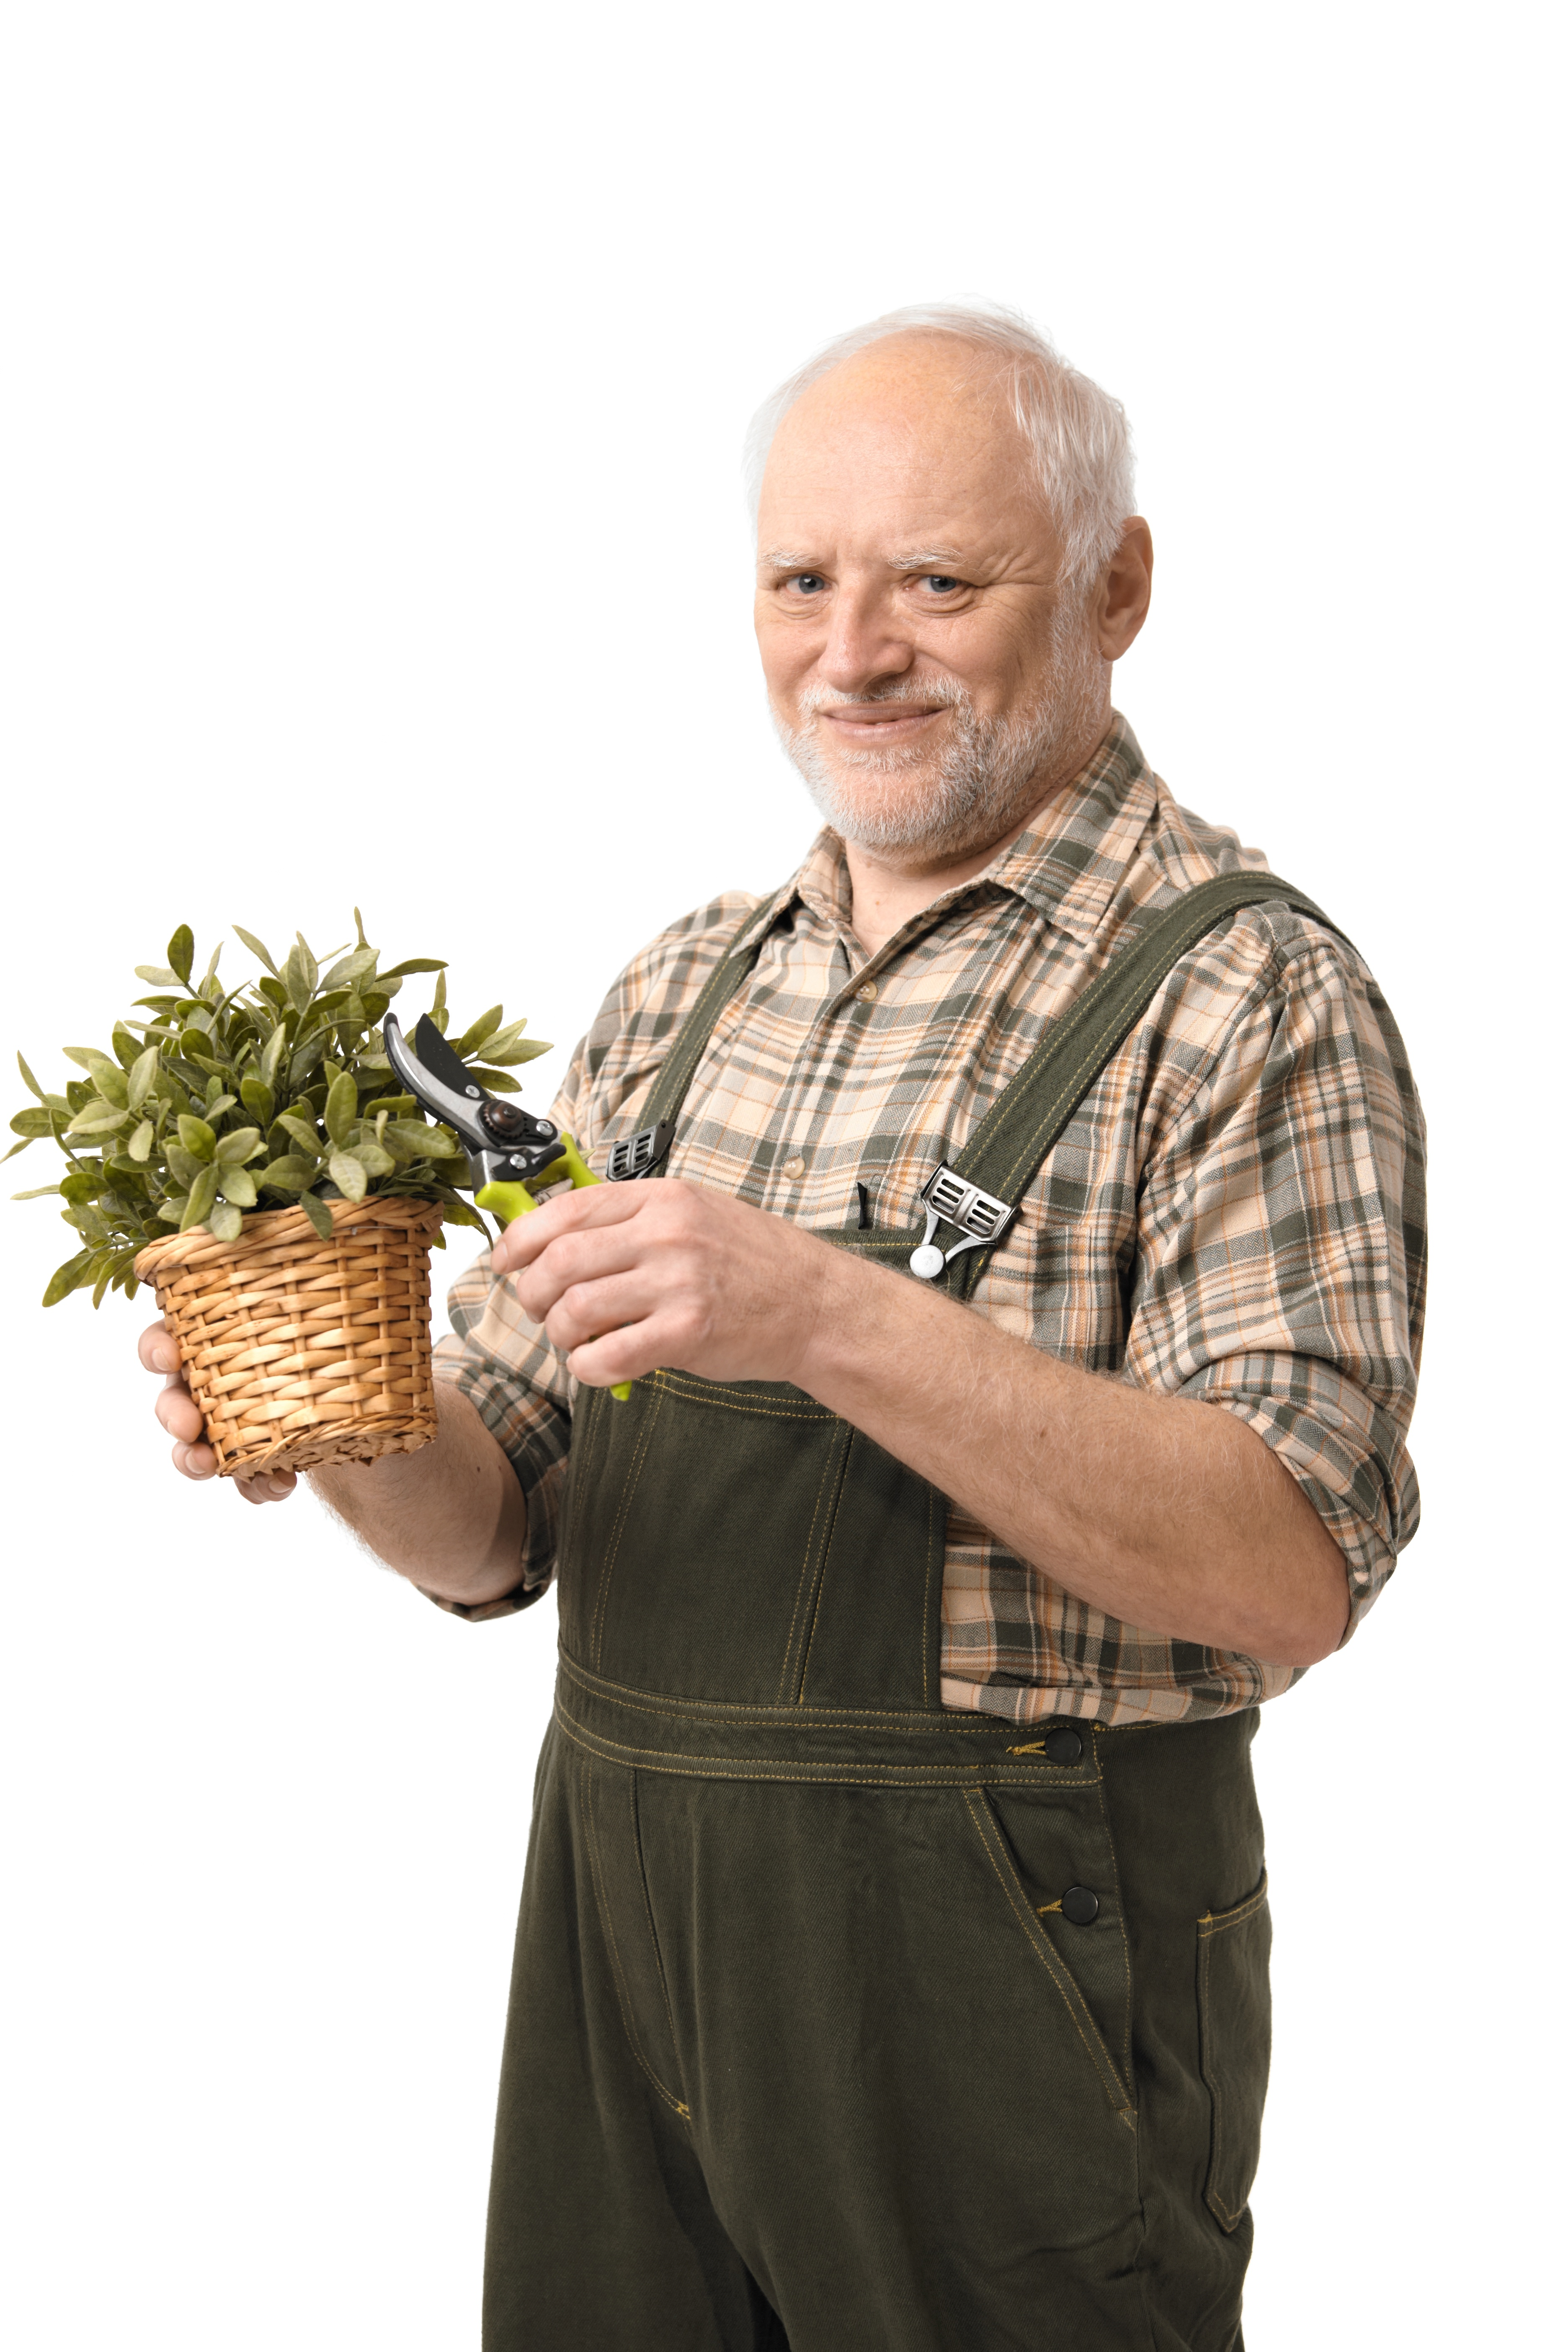
\includegraphics[scale=0.1]{figures/gardener.jpeg}
                \end{figure}
            \end{column}
        \end{columns}
    }
    \only<8>{
        \begin{columns}
            \begin{column}{0.5\textwidth}
                \begin{figure}
                    \centering
                    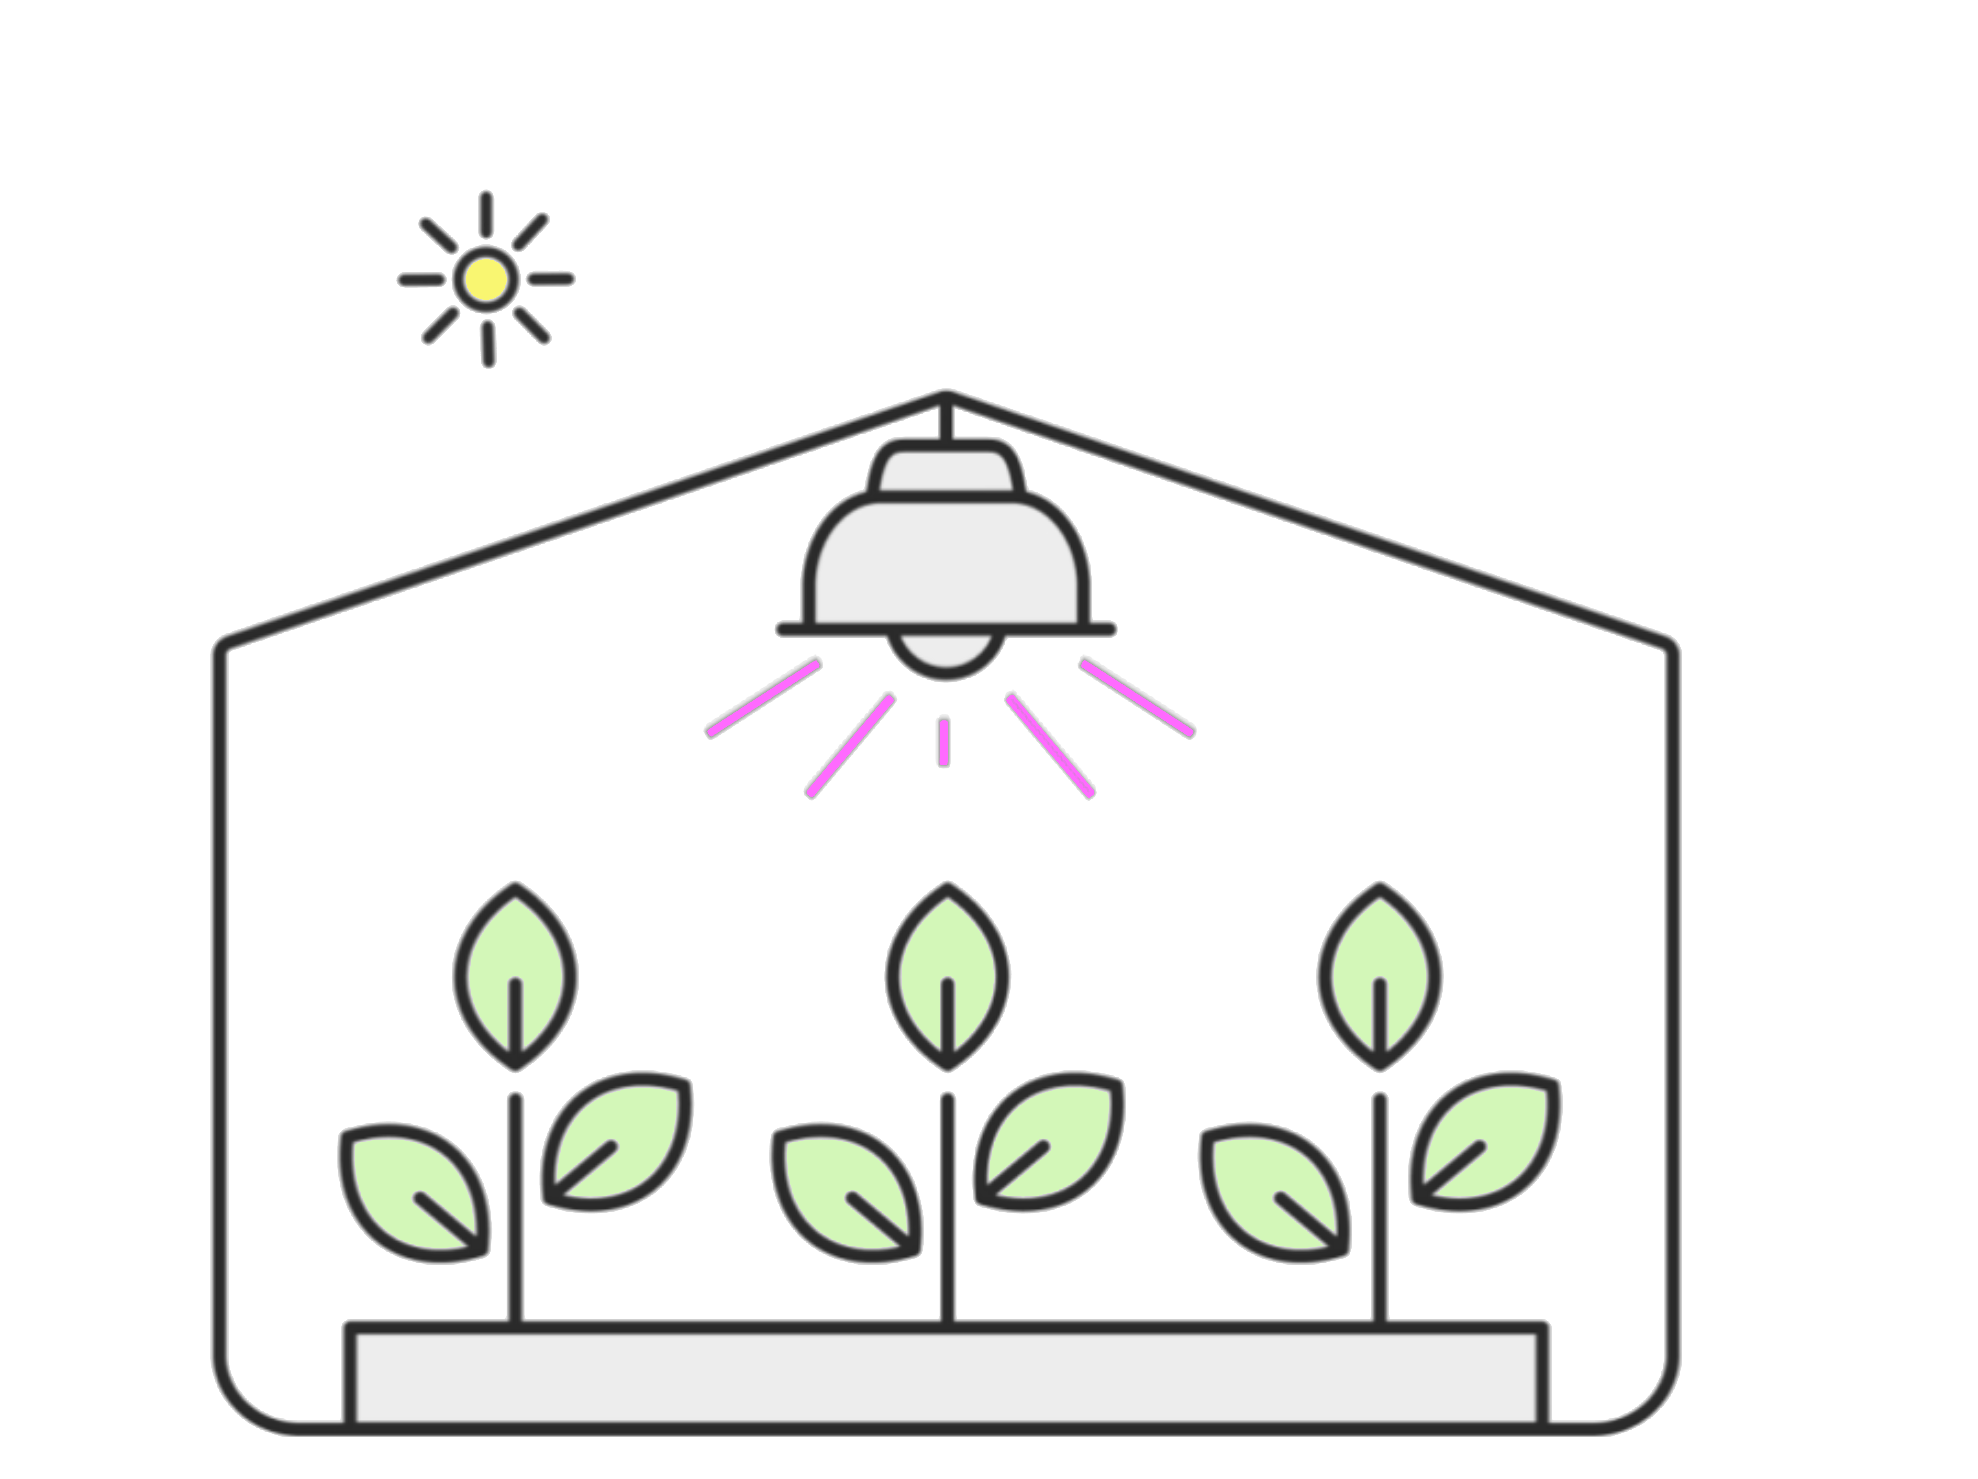
\includegraphics[scale=0.175]{figures/4_lights.png}
                \end{figure}
            \end{column}
            \begin{column}{0.5\textwidth}
                \begin{figure}
                    \centering
                    
\includegraphics[scale=0.1]{figures/computer.jpeg}
                \end{figure}
            \end{column}
        \end{columns}
    }
\end{frame}

\begin{frame}[label=overview]
    \frametitle{Overview}
    
    \begin{figure}
        \centering
        \resizebox{!}{5.5cm}{
            \begin{tikzpicture}[node distance=1cm, font=\footnotesize]
                \node (datacollection) [section] {Data\\Collection};
                \node (plantphysiology) [section, right=of datacollection] {Plant\\Physiology};
                \node (neuralnetwork) [section, right=of plantphysiology] {Neural\\Network};

                \node (costfunction) [section, below=of datacollection, xshift=1.5cm, yshift=-0.5cm] {Cost\\Function};
                \node (constraints) [section, right=of costfunction] {Constraints};

                \node (simulation) [section, below=of costfunction, yshift=-0.5cm] {Simulation};
                \node (results) [section, right=of simulation] {Results};
 
                \node (identification) [chapter, label=above:Identification, fit=(datacollection) (plantphysiology) (neuralnetwork)] {};
                \node (control) [chapter, label=above:Control, fit=(costfunction) (constraints)] {};
                \node (casestudy) [chapter, label=above:{Case Study}, fit=(simulation) (results)] {};

                \draw [arrow] (datacollection) -- (plantphysiology);
                \draw [arrow] (plantphysiology) -- (neuralnetwork);

                \draw [arrow] (identification.east) -| +(0.5,-1) -- +(-9.5,-1) |- (control.west);
                \draw [arrow] (costfunction) -- (constraints);
                \draw [arrow] (control.east) -| +(0.5,-1) -- +(-9.5,-1) |- (casestudy.west);
                \draw [arrow] (simulation) -- (results);
            \end{tikzpicture}
        }
    \end{figure}
\end{frame}